\subsection{Anwendungen mit proprietärer Software}
% \addcontentsline{toc}{subsection}{Anwendungen mit proprietärer Software}
\label{Anwendungen mit proprietärer Software}
Der prorietäre Bereich ist insbesondere durch die Plattformen der globalen Konzerne Microsoft und Amazon geprägt. Beide bieten mit ihren gigantischen Cloudplattformen Azure und Amazon Webservices (\acrshort{AWS}) Lösungen im Bereich \gls{DevOps} an. Diese Lösungen umfassen dabei vor allem Hostingleistungen in den Bereichen Plattform as a Service (\acrshort{PaaS}) und Software as a Service (\acrshort{SaaS}). Das bedeutet, bei diesen Angeboten stellen Microsoft und Amazon wahlweise alle Komponenten bis zur Gesamtplattform oder gleich die vollständige Anwendung (und nur noch die Konfiguration ist vom Anwender durchzuführen).
Gemeinsam ist beiden Lösungen weiterhin, dass die Anbieter jeweils ihre eigenen Tools für die gleichen Anforderungen bereitstellen und natürlich andere Anwendungen des gleichen Konzerns in die Plattformen integrieren.
Im Falle von \acrshort{AWS} geschieht z.B. das zentrale Management einer gesamten Umgebung (und der unterliegenden Infrastruktur) über den Amazon-Systems Manager \cite{aws_systems_manager}, bei Azure verbirgt sich diese Funktion in den Azure Pipelines \cite{azure_devops_loesungen}.
Softwareentwicklung für die cloudbasierte \gls{DevOps}-Umgebung ermöglicht Microsoft über seine konzerneigene Entwicklungsumgebung (\acrshort{IDE}) Visual Studio und die ebenfalls konzerneigene Plattform  GitHub \cite{azure_devops_loesungen}. Amazon bietet hierfür die hauseigene Lösung Codestar \cite{aws_codestar}.
Beide Anbieter stellen einen großen Umfang an Dokumentation, User-Guides, Tutorials, Whitepapern etc. bereit und betonen den einfachen und schnellen Einstieg in die Einrichtung einer \gls{DevOps}-Umgebung (Vgl.\url{https://azure.microsoft.com/de-de/solutions/devops/} und \url{https://aws.amazon.com/de/devops/}).\newline
Es gibt diverse weitere Anbieter, die in diesem Bereich in vergleichbarer Größenordnung aktiv sind und deren Angebote zueinander in Konkurrenz stehen. Neben Azure und \acrshort{AWS} sind u.a. der chinesische Alibaba-Konzern \cite{alibaba_devops} und der englisch-australische Atlassian-Konzern mit seinen Lösungen Jira und Confluence in diesem Bereich aktiv \cite{atlassian_jira_nodate}. 
Weiterhin gibt es in diesem Bereich u.a. Angebote von RedHat Enterprise \cite{redhat_openshift_2017} und IBM, welche vergleichbare Funktionen bieten. IBM ist hier aufgrund eines besonderen Beispiels erwähnt: Auf den Konzern geht die Entwicklung des \gls{LowCode}-Tools NodeRed zurück. NodeRed etabliert auf Basis von NodeJs die Idee der verknüpften Flows und des \glqq{}Infrastructure as Code\grqq (\acrshort{IaC}), ohne gleichzeitig vom Anwender tiefergehende Programmierkenntnisse zu verlangen. IBM hat NodeRed mittlerweile als Opensource-Lösung verfügbar gemacht \cite{nodered_about}.
\begin{center}
    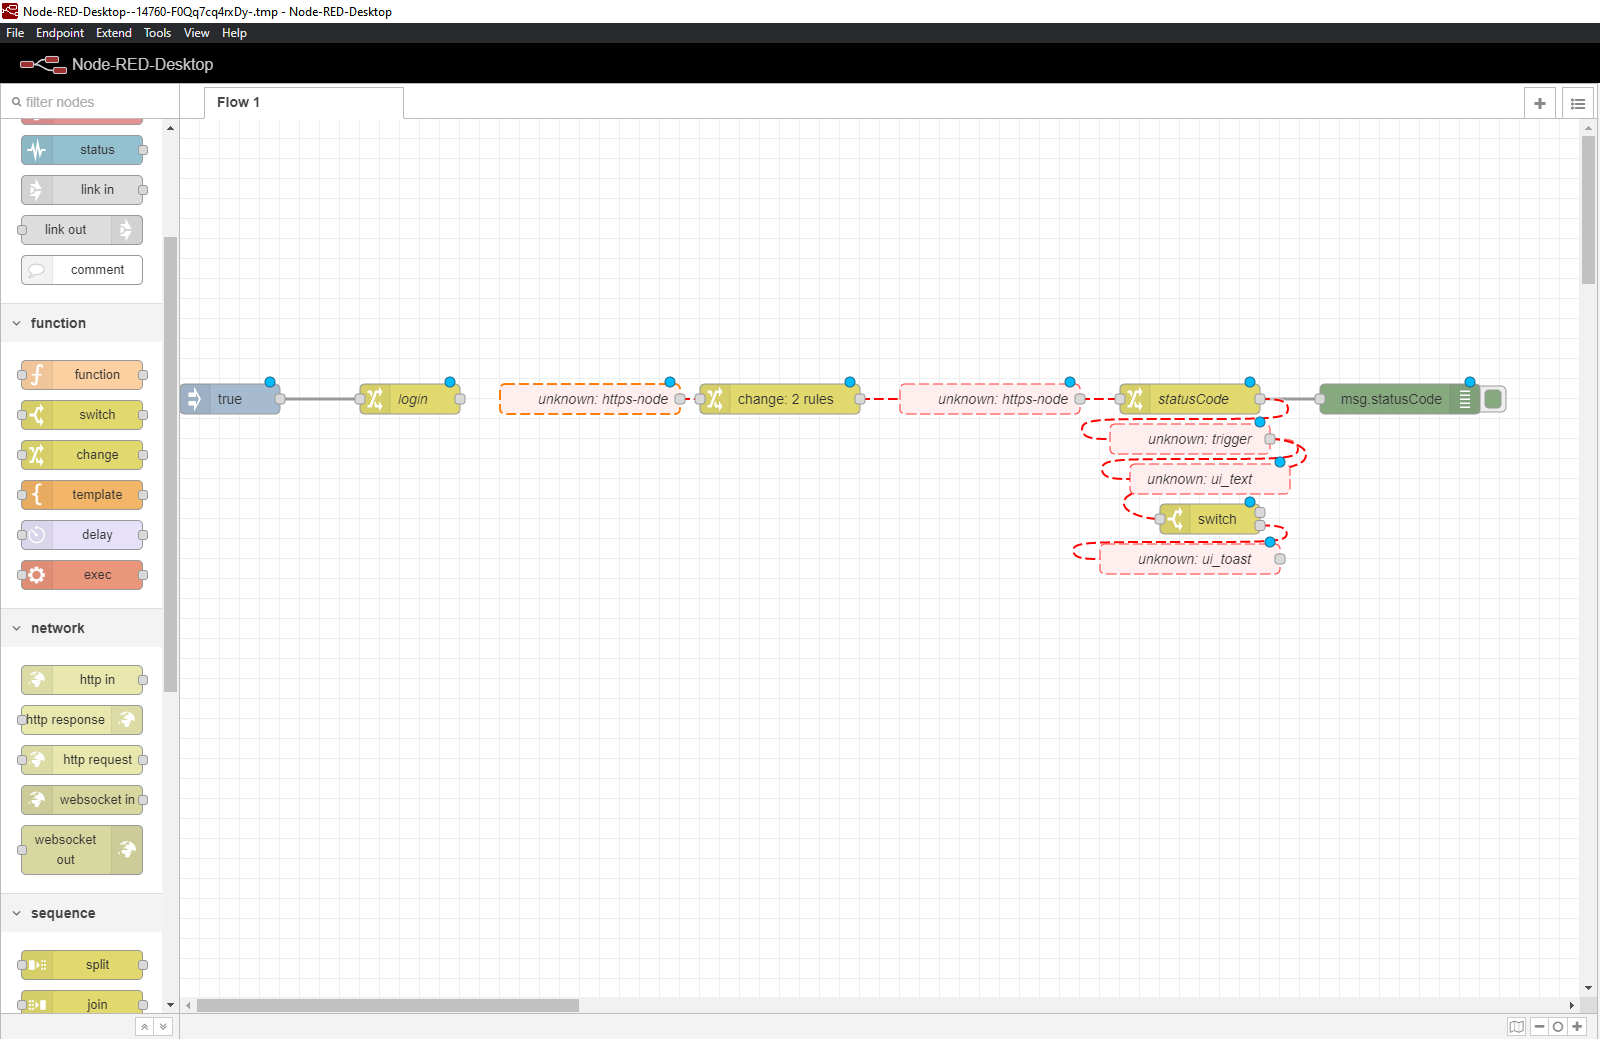
\includegraphics[width=0.6\textwidth]{Grafiken/NodeRed_Flow.png}
    \captionof{figure}{Beispielhafter Flow in der NodeRed-Desktopversion}
    \label{Grafik:Beispielhafter Flow in der NodeRed-Desktopversion}
\end{center}
Zu den vorgestellten proprietären Lösungen kann zusätzlich festgehalten werden, dass diese Plattformen auch zur Senkung der eigenen Betriebs- und Bereitstellungskosten genutzt werden können. Hier kommen die generellen Stärken von Cloudlösungen zum Tragen. Jede Komponente einer \acrshort{CI}/\acrshort{CD}-Plattform, die ausgelagert werden kann, spart eigene Betriebskosten.